\chapter{方案部署及其效果}
\label{cha:experiment}
本章的主要内容为部署防御方案并验证方案有效性。在真实SDN网络中部署防御方案之后,使用不同形式的LDoS攻击对方案进行测试,探测方案的有效性与开销。

\section{实验准备}
\label{chap5:setup}
本文在真实SDN网络中部署防御系统。防御系统使用的SDN控制器为Floodlight控制器。部署了防御系统的控制器被部署在一个服务器上,该服务器的配置为Intel Xeon Quad-Core CPU E5504和4GB的RAM。在系统中我们使用了OpenFlow商业硬件交换机(EdgeCore AS4610-54T)作为真实SDN网络使用的硬件交换机。硬件交换机的端口转发速率最高能够可达到1Gbps,本文将最大转发速率标记为$R_m$。为了验证系统有效性,本文使用C代码生成不同$T$与$L$的LDoS攻击。并且使用Python代码完成分布式LDoS攻击的部署。

图\ref{fig:topology}展示了实验使用的SDN网络拓扑图。它有7个主机和3个OpenFlow硬件交换机组成。其中2个主机为攻击主机,5个主机为正常的主机。在实验中,$h_1$发送正常流量作为背景流量并由$h_5$接收,$h_3$与$h_6$之间建立TCP连接。$h_2$和$h_4$被设置为LDoS攻击的发送端,由$h_7$接收他们发送的LDoS攻击流量。对于攻击者$h_2$和$h_4$的不同配置可以得到单一攻击源的LDoS攻击,也可以得到分布式LDoS攻击。

%对于这个网络,LDoS攻击流的目的是完全占用$S_2$与$S_3$之间连接的带宽致使$S_2$的队列被拥塞造成$h_1$

\begin{figure}
    \centering
    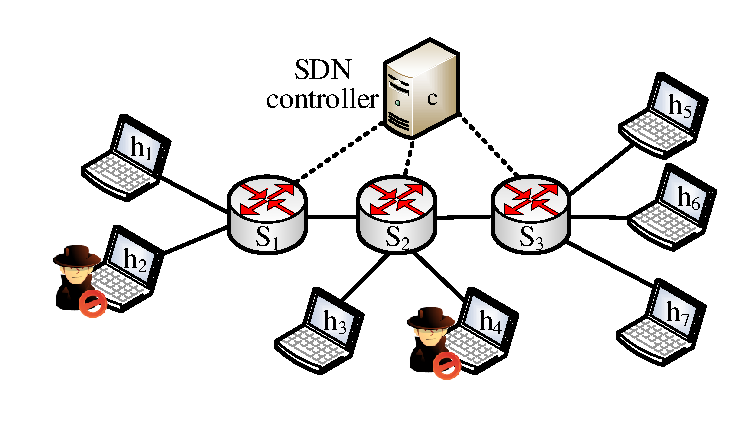
\includegraphics[scale=1]{topology}
    \caption{实验使用拓扑图}
    \label{fig:topology}
\end{figure}


\section{基于带宽保障的方案}

\section{基于动态周期性检测的防御方案}
\label{chap5:expperioddetection}
在系统部署了基于动态周期性检测的方案之后,本文通过对检测精确度和方案的开销对方案进行全方位的讨论和分析,对方案的有效性进行评价。对方案的评估包括一个主机完成LDoS攻击和两个主机完成LDoS攻击两种形式。

\subsection{精确度分析}
\label{chap5:accuracy}
这个部分主要分析基于动态周期性检测的防御方案的各个模块的准确性和稳定性。首先,本文对异常检测模块成功检测到端口异常的成功率做实验进行分析。然后,本文计算了攻击定位模块推断出的LDoS攻击周期与真正的LDoS周期之间的误差。接下来,本文通过实验获得了经过受影响端口与经过端口流量的平均欧式距离的概率密度函数(Probability Density Function,PDF),并在此基础上,找到了用于判断攻击流的阈值。最后,本文探索了平均欧式方法判断攻击流的准确度。

异常检测模块在异常端口处检测到可能的LDoS攻击时才会激活攻击定位模块对异常端口进行进一步的分析,因此,该模块在LDoS攻击存在的情况下检测到端口吞吐量异常的成功率直接关键到LDoS攻击能否被系统检测,因此,本文对异常检测模块的参数$\alpha$和$M$进行了探讨。

% alpha,M两个参数进行分析讨论,出图,(1-2页)

% alpha和LDoS识别率,M作为稳定参数,多次取值,准确识别LDoS的图

% alpha和误判率,M作为稳定参数,多次取值,正常流判断为LDoS流


攻击定位模块的第一步是对序列进行二值化,本文将阈值$\beta$设为0.8。接下来,本文通过对异常端口的计数器获取的数据推测LDoS攻击的周期。在获得二值化序列之后,本文对该序列进行周期性的推测。如果在异常的端口处存在LDoS攻击流,则推断出的序列周期将会是一个正数。但是,如果端口不存在LDoS攻击流,则推断出的序列周期将会为0。为了获得攻击定位模块推断的周期准确度,本文比较通过序列推断出的周期与LDoS攻击流的真实周期,得到了推断的周期误差。

\begin{figure}
    \centering
    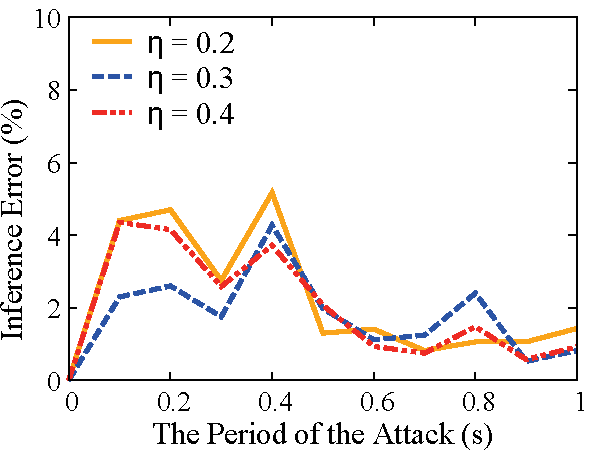
\includegraphics[scale=1.0]{period}
    \caption{推断误差}
    \label{fig:period}
\end{figure}

图\ref{fig:period}展示了不同LDoS攻击的周期下,攻击定位模块推断的周期与真实LDoS攻击的周期的相对误差。此处使用算法\ref{alg:port_locate}来预测LDoS攻击的周期。实验中,我们将LDoS攻击的突发速率$R$置为1Gbps。对于算法的参数,考虑系统的带宽和识别率保证,本文设定$T_e$为0.005,$T_i$为0.64,$\epsilon$ = 0.01。为了查看算法对LDoS攻击周期的适应性,在LDoS攻击的周期从0.1上升至1s的情况下,使用攻击检测模块对不同$\eta$值的LDoS攻击的周期进行预测。除此之外,还使用洪泛攻击测试算法。每次使用5秒获取端口的数据进行测试。实验的结果表示,攻击检测模块能够确认异常端口上的LDoS攻击,同时,推测出来的周期也存在一定的误差,但是,推断出的相对误差最多不超过6\%。LDoS攻击不存在(洪泛攻击)的情况下,由于洪泛攻击没有周期,而推断出的周期为0,因此,在0点处,误差为0。在大多数情况下,在LDoS攻击的周期值比较小的时候,相对误差会比较大。攻击检测模块的绝对误差在0至30毫秒之间,随着算法的周期不断变大,攻击检测模块的相对误差也相应的减小。通过这次实验也获得了相应的$T_s$。攻击定位模块在确认了LDoS攻击在异常端口存在之后,使用了$T_s$作为采样间隔获取流表规则上的计数器数据用以对识别攻击流。

在确认端口受LDoS攻击影响之后,控制器以$T_s$的采样间隔同时获取受影响端口序列与经过该端口的流的信息,在通过二值化之后对二值化流量做进一步分析。在LDoS攻击的$T$设为1秒,$L$设为0.2秒的时候,控制器以$T_s$为0.2s获取流表规则计数器上的数据,则可以获得受影响端口、正常数据流和LDoS攻击流的吞吐量二值化序列。如图\ref{fig:binary-sequence}所示,三者的吞吐量二值化序列的形状是完全不同的,受影响端口的二值化序列的形状与LDoS攻击流的二值化序列更加相近,而背景流量的形状则与受影响端口的二值化序列不相似。在LDoS突发出现的时候,即图中LDoS攻击的二值化吞吐量值为1的时候,受影响端口的二值化吞吐量也为1,此时,背景流量的二值化吞吐量为0,因为,在LDoS攻击的突发时间里的情况下,交换机转发的背景流量低于没有LDoS攻击时的最高速率,在二值化的时候把该时刻的值置为0。在LDoS攻击存在的情况下,受影响端口统计的吞吐量序列最大值$S_m$即为$R_m$,因此,受影响端口统计的吞吐量序列中流量的速率在LDoS攻击不存在的情况下基本低于$\beta * S_m$。受影响端口在LDoS攻击不存在的情况下的二值化吞吐量基本为0。从此图中也可以,使用平均欧式距离区分LDoS攻击流与背景流是可行的。



\begin{figure}
    \centering
    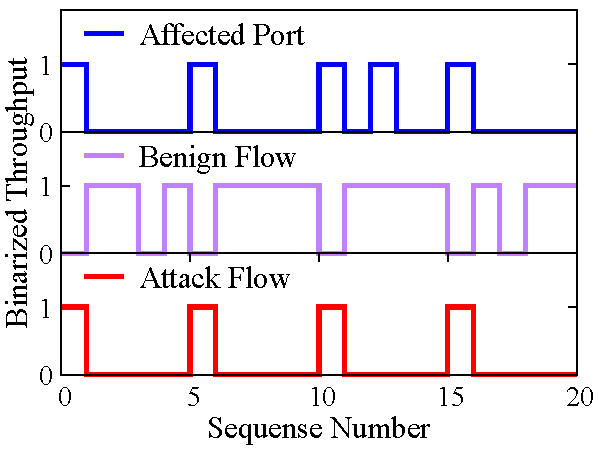
\includegraphics[scale=1.3]{binary-sequence}
    \caption{二值化吞吐量序列}
    \label{fig:binary-sequence}
\end{figure}



为了获得合适的阈值$\gamma$来识别攻击流,受影响端口的二值化序列与经过该端口的数据流的平均欧式距离的概率密度函数是必须的,但是一个攻击源与多个攻击源的情况不同,因此,需要多次试验来分析不同的情况下。LDoS攻击流平均欧氏距离与正常数据流的平均欧氏距离是完全不同的。在经过了二值化之后,LDoS攻击流的二值化序列与受影响端口统计的二值化序列的平均欧式距离比正常流量小很多,因此,找到合适的阈值$\gamma$,就可以识别攻击流。首先,考虑验证系统对于大部分情况的适应性,只用一个固定的$T$是不足够的,所以,LDoS攻击的$T$随机从0.8至1.5之前取值,因为LDoS攻击的$T$取值过大会是TCP流无法进入超时重传状态。接下来,考虑到$L$的取值不应过小或者过大,设置LDoS攻击的突发长度$L$从0.1至0.4之间随机取值。如果$L$太小,则无法造成TCP流丢包,则无法达到LDoS攻击的效果。但是,如果$L$的取值过大,则平均速率会很高,容易被洪泛服务拒绝攻击的检测方式检测到。最后,考虑交换机最大转发速率为1Gbps,所以,LDoS攻击的突发速率$R$设为1Gbps已经是能够达到的最大速率了,如果突发速率更高则可能造成LDoS攻击自身丢包过多,反而容易被检测到。考虑到需要有背景流量作为良性的流量干扰防御系统以验证攻击定位模块的有效性,$h_1$生成了100条良性流作为背景流量发送给$h_5$。

本文先分析一个攻击源生成LDoS攻击的情况。以$h_2$作为攻击源发送LDoS攻击流,$h_4$不发送攻击流量。经过多次试验,获得图\ref{fig:PDF-single}作为单攻击源的概率密度函数。可以看到,LDoS攻击流的二值化序列与受影响端口的二值化序列的平均欧式距离的主要分布在0.2与0.4之间,平均值为0.3。而正常流的二值化序列与受影响端口的二值化序列的平均欧式距离的主要分布在0.44至0.84之间,平均值为0.64。绝大部分情况下,LDoS攻击流的二值化序列与受影响端口的二值化序列的平均欧式距离比正常流的二值化序列与受影响端口的二值化序列的平均欧式距离小。因为在LDoS攻击突发存在的情况下,端口转发的主要流量为LDoS攻击。而没有LDoS攻击攻击存在的时候,正常流公平竞争带宽,因此,速率更高,在突发不存在的时候,二值化吞吐量值为1,受影响端口的二值化序列为0,刚好相反,因此平均欧式距离更大。从图\ref{fig:PDF-single}中可以看到一个清晰的区分点,即$MED$为0.42。该点可以作为识别单攻击源中LDoS攻击流的阈值。

\begin{figure}
    \begin{minipage}[t]{0.49\linewidth}
        \centering
        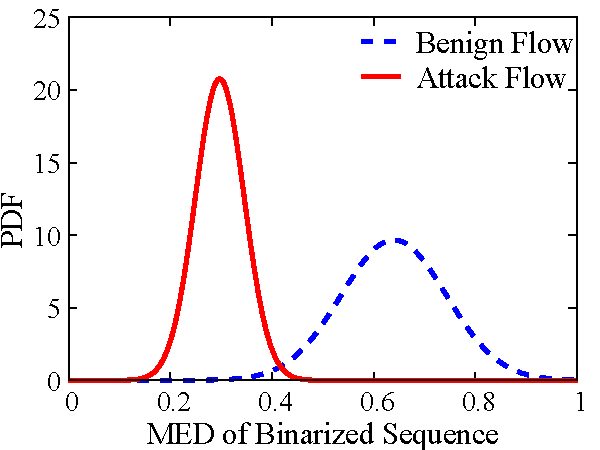
\includegraphics[scale=0.7]{distribution}
        \caption{\small{单攻击源的平均欧式距离的PDF}}
        \label{fig:PDF-single}
    \end{minipage}
    \begin{minipage}[t]{0.49\linewidth}
        \centering
        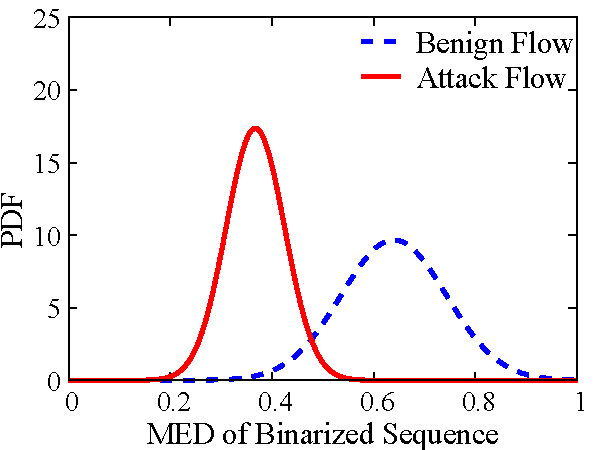
\includegraphics[scale=0.7]{distribution1}
        \caption{\small{分布式方案一平均欧式距离的PDF}}
        \label{fig:PDF-2h-mod1}
    \end{minipage}

    \begin{minipage}[t]{0.49\linewidth}
        \centering
        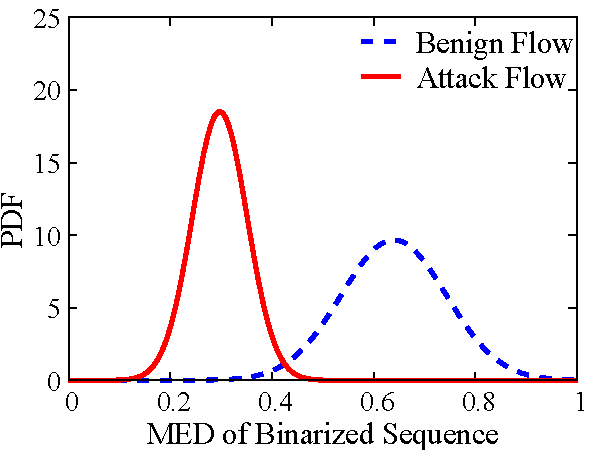
\includegraphics[scale=0.7]{distribution2}
        \caption{\small{分布式方案二平均欧式距离的PDF}}
        \label{fig:PDF-2h-mod2}
    \end{minipage}
        \begin{minipage}[t]{0.49\linewidth}
        \centering
        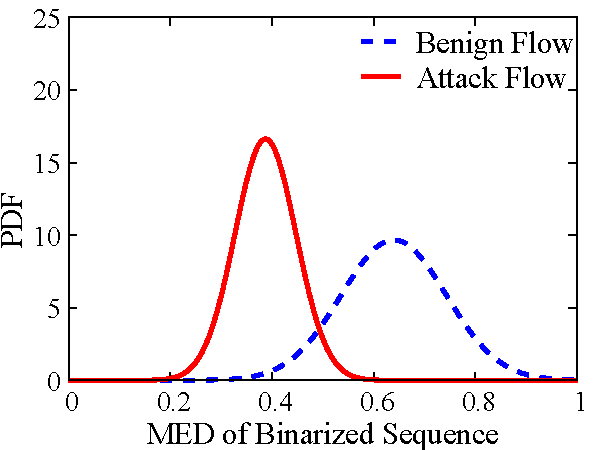
\includegraphics[scale=0.7]{distribution3}
        \caption{\small{分布式方案三平均欧式距离的PDF}}
        \label{fig:PDF-2h-mod3}
    \end{minipage}
\end{figure}

在获得单攻击源的平均欧式距离的概率分布函数之后,可以确认使用平均欧氏距离的方法确实可以区分攻击流与正常流。接下来,对多攻击源分布式LDoS攻击进行区分,因此,以$h_2$和$h_4$同时作为攻击源发送LDoS攻击流,分布式LDoS攻击的三种方案产生流量,获得相应的平均欧式距离的概率密度函数。两主机以分布式方案一的方式产生LDoS攻击的流量,获得图\ref{fig:PDF-2h-mod1}。从图中可看出,与单攻击源不同,LDoS攻击流的二值化序列与受影响端口的二值化序列的平均欧式距离的主要分布发生了变化,主要分布在0.24至0.48,平均值为0.36,而正常流的二值化序列与受影响端口的二值化序列的平均欧式距离的主要分布在0.45至0.85之间,平均值为0.65。以方案一平均欧式距离的分布函数平均值变大,因为在受影响端口处统计的突发包括了两个主机的突发流量,而使用流表规则统计的数据只包含一个流的数据,因此,计算出的平均欧式距离统计的平均值相较于单攻击源的平均欧式距离统计的平均值更大。因此,对于方案一而言,最佳的区分点为0.47。

当两个主机以分布式方案二的方式产生LDoS攻击的流量,获得图\ref{fig:PDF-2h-mod2}。从图中可看出,LDoS攻击流的二值化序列与受影响端口的二值化序列的平均欧式距离的主要分布与

% \begin{figure}
%     \centering
%     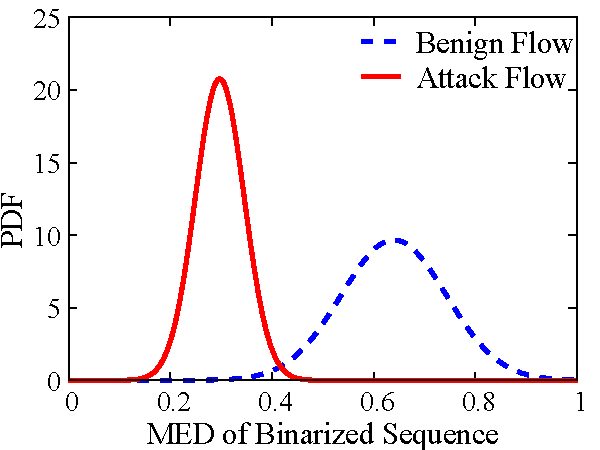
\includegraphics[scale=0.6]{distribution}
%     \caption{平均欧式距离的概率密度函数}
%     \label{fig:PDFofMED}
% \end{figure}



%二值化后数据对比







